\section{Methodik}
\label{sec:method}

In diesem Kapitel wird der in dieser Arbeit verfolgte methodische Ansatz zur
semi-supervisierten Videoannotation beschrieben. Ziel ist es, den manuellen
Annotierungsaufwand bei video-basierten Luftaufnahmen deutlich zu reduzieren,
ohne dabei die Qualität der erzeugten Annotationen wesentlich zu beeinträchtigen.
Hierzu wird ein iterativer Ansatz vorgestellt, der Transfer Learning,
Objektverfolgung und Pseudo-Labeling miteinander kombiniert.

Der zentrale Gedanke des Ansatzes besteht darin, lediglich eine kleine Teilmenge
der Videoframes manuell zu annotieren und diese als Ausgangspunkt für das Training
eines vortrainierten Objekterkennungsmodells zu nutzen. Auf Basis dieses Modells
werden anschließend nicht annotierte Zwischenframes automatisch analysiert. Die
dabei erzeugten Detektionen werden mithilfe eines Tracking-Verfahrens zeitlich
verknüpft, um konsistente Objekttrajektorien über mehrere Frames hinweg zu
erhalten.

Die aus der Objektverfolgung resultierenden Informationen werden genutzt, um
automatisch zusätzliche Annotationen in Form von sogenannten Pseudo-Labels zu
erzeugen. Durch den Einsatz einfacher heuristischer Kriterien, wie
Konfidenzschwellwerten und minimalen Tracking-Dauern, wird die Qualität dieser
Pseudo-Labels kontrolliert. Die so erweiterten Annotationen dienen anschließend
als Trainingsdaten für eine erneute Modellanpassung im Sinne eines iterativen
Self-Training-Prozesses.

Der beschriebene Ansatz ist modular aufgebaut und erlaubt es, einzelne
Komponenten wie die Anzahl der Iterationen, die Tracking-Strategie oder die
Filterkriterien flexibel anzupassen. Dadurch eignet sich der vorgestellte
Ansatz insbesondere für reale Anwendungsszenarien mit begrenzten manuellen
Annotierungsressourcen und großen Mengen an Videodaten.


\newpage

\usetikzlibrary{shapes.geometric, arrows.meta, positioning, calc}

\begin{figure}[htbp]
    \centering
    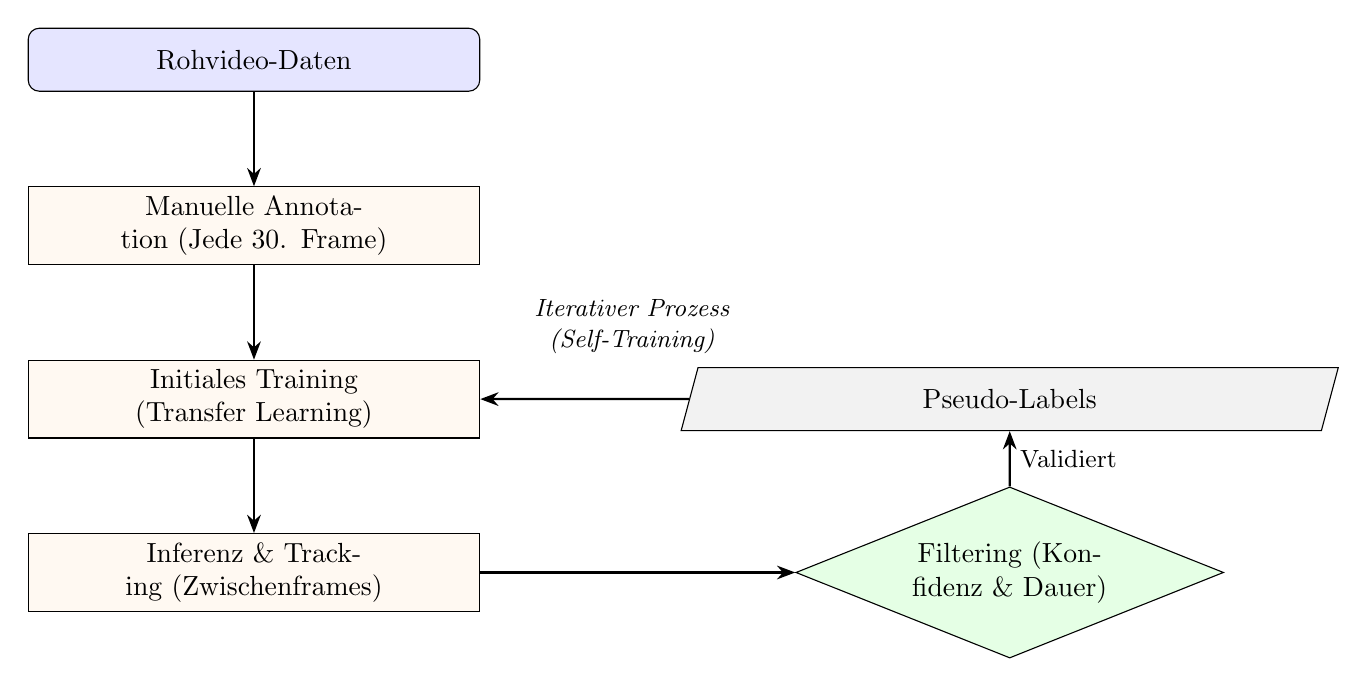
\begin{tikzpicture}[
            % Yatay mesafeyi (4.5cm) ve dikey mesafeyi (1.2cm) ayarladık
            node distance=1.2cm and 4cm,
            auto,
            % Kutuların genişliğini tek satıra sığacak şekilde 5.5cm yaptık
            startstop/.style={rectangle, rounded corners, draw, fill=blue!10, text width=5.5cm, align=center, minimum height=0.8cm},
            process/.style={rectangle, draw, fill=orange!5, text width=5.5cm, align=center, minimum height=0.8cm},
            decision/.style={diamond, draw, fill=green!10, text width=3.5cm, align=center, inner sep=0pt, aspect=2.5},
            data/.style={trapezium, draw, fill=gray!10, trapezium left angle=75, trapezium right angle=105, text width=4.5cm, align=center, minimum height=0.8cm},
            arrow/.style={-Stealth, thick}
        ]

        % Düğümler (Nodes) - Metinler artık tek satır
        \node (start) [startstop] {Rohvideo-Daten};

        \node (manual) [process, below=of start] {Manuelle Annotation (Jede 30. Frame)};

        \node (train) [process, below=of manual] {Initiales Training (Transfer Learning)};

        \node (inference) [process, below=of train] {Inferenz \& Tracking (Zwischenframes)};

        % Sağ taraf
        \node (filter) [decision, right=of inference] {Filtering (Konfidenz \& Dauer)};

        \node (pseudo) [data] at (train -| filter) {Pseudo-Labels};

        % Oklar (Arrows)
        \draw [arrow] (start) -- (manual);
        \draw [arrow] (manual) -- (train);
        \draw [arrow] (train) -- (inference);
        \draw [arrow] (inference) -- (filter);
        \draw [arrow] (filter) -- node[right, font=\small] {Validiert} (pseudo);
        \draw [arrow] (pseudo) -- (train);

        % Döngü Etiketi
        \node [font=\small\itshape, text width=4cm, align=center, anchor=south]
        at ($(pseudo.north)!0.5!(train.north)$) {Iterativer Prozess (Self-Training)};

    \end{tikzpicture}
    \caption{Methodischer Ablauf: Iterative Video-Annotation mittels Transfer Learning, Tracking und Pseudo-Labeling.}
    \label{fig:methodik_workflow}
\end{figure}

\subsection{Gesamtübersicht des Ansatzes}

Der in dieser Arbeit verfolgte Ansatz zielt darauf ab, den manuellen Aufwand für die
Annotation video-basierter Luftaufnahmen deutlich zu reduzieren. Hierzu wird ein
semi-supervisiertes Verfahren eingesetzt, das Transfer Learning, Objektverfolgung
sowie automatische Label-Propagation kombiniert. Der Ansatz ist insbesondere für
Szenarien geeignet, in denen große Mengen an Videodaten vorliegen, eine vollständige
manuelle Annotation jedoch nicht praktikabel ist.

Ausgangspunkt des Verfahrens ist eine begrenzte Menge manuell annotierter Videoframes,
die in regelmäßigen Abständen aus den Rohvideos extrahiert werden. Diese sparsam
annotierten Frames dienen als Trainingsgrundlage für ein vortrainiertes
Objekterkennungsmodell. Das Modell wird nicht von Grund auf neu trainiert, sondern im
Sinne des Transfer Learnings an die domänenspezifischen Inhalte der Luftaufnahmen
angepasst.

Das initial trainierte Modell wird anschließend auf nicht annotierte Zwischenframes
angewendet, um potenzielle Objekte automatisch zu detektieren. Da es sich um
Videodaten handelt, weisen die Detektionen eine zeitliche Abhängigkeit zwischen
aufeinanderfolgenden Frames auf. Um diese zeitliche Konsistenz gezielt auszunutzen,
wird ein Objektverfolgungsverfahren eingesetzt, das Detektionen über mehrere Frames
hinweg miteinander verknüpft und stabile Objekttrajektorien erzeugt.

Auf Basis der verfolgten Objekttrajektorien werden zusätzliche Annotationen in Form
von sogenannten Pseudo-Labels generiert. Um die Qualität dieser automatisch erzeugten
Labels sicherzustellen, kommen einfache heuristische Filter zum Einsatz, etwa
Schwellwerte für Detektionskonfidenzen oder Mindestdauern von Objekttracks. Die so
gewonnenen Pseudo-Labels erweitern den ursprünglichen Trainingsdatensatz.

Dieser erweiterte Datensatz kann anschließend für eine erneute Modellanpassung
verwendet werden. Durch eine optionale iterative Wiederholung dieses Prozesses wird
ein Self-Training-Ansatz realisiert, der es erlaubt, die Leistungsfähigkeit des
Objekterkennungsmodells schrittweise zu verbessern, ohne den manuellen
Annotierungsaufwand signifikant zu erhöhen. Die einzelnen Komponenten des Ansatzes
sind modular aufgebaut und können abhängig von den experimentellen Ergebnissen
angepasst oder vereinfacht werden.


\begin{figure}[htbp]
    \centering
    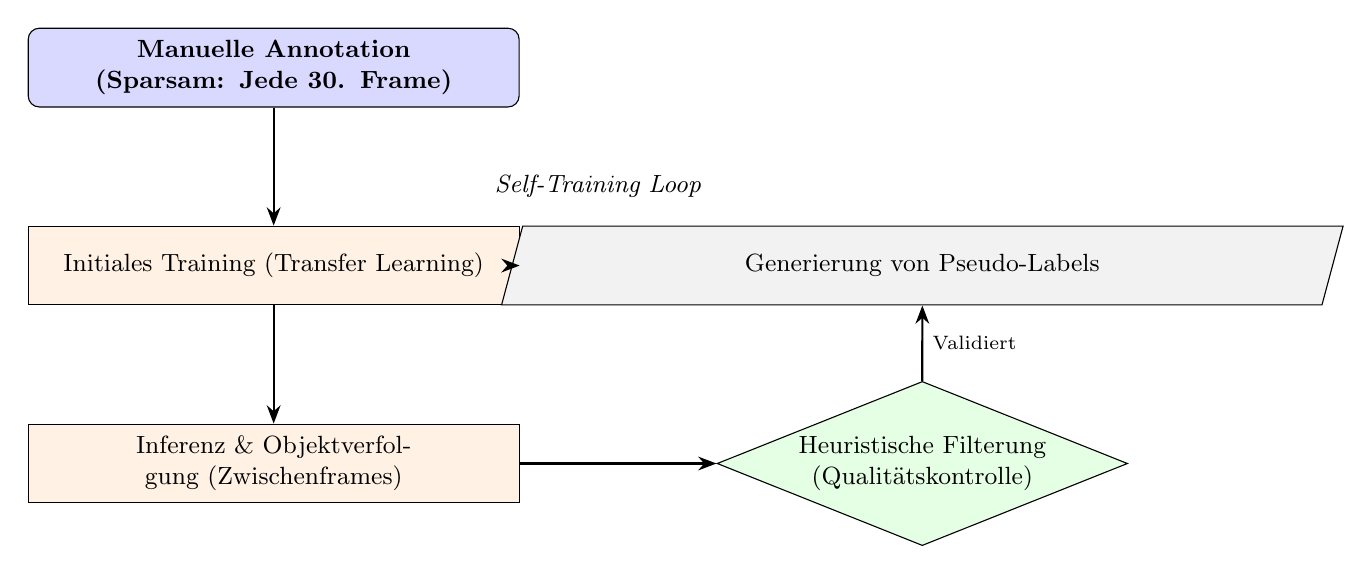
\begin{tikzpicture}[
            node distance=1.5cm and 2.5cm,
            auto,
            manual_style/.style={rectangle, rounded corners, draw, fill=blue!15, text width=6cm, align=center, minimum height=1cm, font=\small\bfseries},
            auto_style/.style={rectangle, draw, fill=orange!10, text width=6cm, align=center, minimum height=1cm, font=\small},
            decision_style/.style={diamond, draw, fill=green!10, text width=3.5cm, align=center, inner sep=0pt, aspect=2.5, font=\small},
            data_style/.style={trapezium, draw, fill=gray!10, trapezium left angle=75, trapezium right angle=105, text width=5cm, align=center, minimum height=1cm, font=\small},
            line/.style={-Stealth, thick}
        ]

        % Dikey Ana Akış (Manual -> Initial Training)
        \node (manual) [manual_style] {Manuelle Annotation (Sparsam: Jede 30. Frame)};
        \node (train) [auto_style, below=of manual] {Initiales Training (Transfer Learning)};
        \node (inference) [auto_style, below=of train] {Inferenz \& Objektverfolgung (Zwischenframes)};

        % Sağ Taraf (Iteratif Döngü)
        \node (filter) [decision_style, right=of inference] {Heuristische Filterung \\ (Qualitätskontrolle)};
        \node (pseudo) [data_style] at (train -| filter) {Generierung von Pseudo-Labels};

        % Bağlantılar
        \draw [line] (manual) -- (train);
        \draw [line] (train) -- (inference);
        \draw [line] (inference) -- (filter);
        \draw [line] (filter) -- node[right, font=\scriptsize] {Validiert} (pseudo);
        \draw [line] (pseudo) -- (train);

        % Döngü Açıklaması
        \node [font=\small\itshape, text width=4cm, align=center] at ($(pseudo.north)!0.5!(train.north) + (0,0.5)$) {Self-Training Loop};

    \end{tikzpicture}
    \caption{Gesamtübersicht des semi-supervisierten Ansatzes zur iterativen Videoannotation.}
    \label{fig:methodik_overall}
\end{figure}

\subsection{Basismodell und Transfer Learning}

Als Basismodell wird in dieser Arbeit ein YOLO-basiertes Objekterkennungsmodell
verwendet, das für allgemeine Objekterkennungsaufgaben vortrainiert wurde. Modelle
der YOLO-Familie zeichnen sich durch ihren einstufigen Aufbau aus, bei dem
Objektlokalisierung und Klassifikation in einem gemeinsamen Vorwärtsschritt
durchgeführt werden. Dadurch eignen sie sich besonders für video-basierte
Anwendungsszenarien, in denen sowohl eine hohe Detektionsgenauigkeit als auch eine
effiziente Inferenz erforderlich sind.

Das Training des Modells erfolgt nicht von Grund auf neu. Stattdessen werden die
vortrainierten Modellgewichte als Ausgangspunkt genutzt und im Rahmen des Transfer
Learnings an die domänenspezifischen Eigenschaften der verwendeten Luftaufnahmen
angepasst. Diese Entscheidung basiert auf der Beobachtung, dass insbesondere bei
begrenzter Verfügbarkeit manuell annotierter Trainingsdaten ein Training mit
zufälliger Initialisierung zu instabilen Lernverläufen und einer erhöhten
Überanpassung führen kann. Durch die Nutzung vortrainierter Gewichte können bereits
gelernte allgemeine visuelle Merkmale, wie Kanten, Texturen und einfache Formen,
direkt übernommen werden.

Im Rahmen des Transfer-Learning-Prozesses werden die vorhandenen Modellgewichte als
Initialisierung verwendet, während die Ausgabeschichten an die im Ziel-Datensatz
definierten Objektklassen angepasst werden. Das Modell wird anschließend mithilfe
der sparsam annotierten Videoframes feinjustiert. Dabei liegt der Fokus nicht auf
einer vollständigen Neuanpassung aller Merkmale, sondern auf der schrittweisen
Anpassung höherer Repräsentationsebenen an die spezifischen visuellen Eigenschaften
von UAV-Aufnahmen, wie veränderte Perspektiven, geringe Objektgrößen und komplexe
Hintergrundstrukturen.

Durch dieses Vorgehen wird erreicht, dass das Modell bereits in frühen
Trainingsphasen sinnvolle Detektionen erzeugen kann, obwohl nur eine begrenzte
Anzahl manuell annotierter Beispiele zur Verfügung steht. Diese Eigenschaft ist
insbesondere für den weiteren Verlauf des vorgeschlagenen Ansatzes von Bedeutung,
da das initial trainierte Modell als Grundlage für die automatische Annotation
nicht beschrifteter Zwischenframes dient.

Zusammenfassend stellt das eingesetzte Transfer-Learning-Verfahren einen zentralen
Baustein des gesamten Ansatzes dar. Es ermöglicht eine stabile Initialisierung des
Objekterkennungsmodells, reduziert den Bedarf an umfangreichen manuellen
Annotationen und schafft die Voraussetzung für die nachgelagerten Schritte der
Objektverfolgung, Pseudo-Label-Generierung und iterativen Modellanpassung.
\subsection{Automatische Annotation durch Pseudo-Labeling}

Im nächsten Schritt des vorgeschlagenen Ansatzes wird das initial mittels
Transfer Learning trainierte Objekterkennungsmodell eingesetzt, um nicht manuell
annotierte Zwischenframes automatisch zu analysieren. Die dabei erzeugten
Detektionen werden als sogenannte Pseudo-Labels interpretiert und bilden die
Grundlage für eine schrittweise Erweiterung des Trainingsdatensatzes.

Ziel des Pseudo-Labeling-Verfahrens ist es, ausgehend von einer begrenzten Anzahl
manuell annotierter Frames zusätzliche Trainingsdaten zu generieren. Auf diese
Weise soll untersucht werden, ob nicht manuell annotierte Zwischenframes zur
Erweiterung der Datenbasis genutzt werden können, ohne den manuellen
Annotierungsaufwand proportional zur Datenmenge zu erhöhen. Die vom Modell
erzeugten Vorhersagen werden jedoch nicht ungefiltert übernommen, sondern einer
gezielten Qualitätskontrolle unterzogen.

In der detection-basierten Pseudo-Labeling-Stufe erfolgt die Auswahl gültiger
Pseudo-Labels primär anhand der Detektionskonfidenz. Ein automatisch erzeugtes
Detektionsergebnis \(d\) wird nur dann als Pseudo-Label in den Trainingsdatensatz
übernommen, wenn seine Konfidenz einen definierten Schwellenwert überschreitet.
Formal lässt sich die Menge der akzeptierten detection-basierten Pseudo-Labels
wie folgt beschreiben:

\[
    L_{\text{pseudo}} =
    \{ d \in D \mid score(d) \geq \tau_{\text{conf}} \}
\]

Dabei bezeichnet \(D\) die Menge aller automatisch erzeugten Detektionen,
\(score(d)\) die Konfidenz einer einzelnen Detektion und \(\tau_{\text{conf}}\)
den minimal erforderlichen Konfidenzschwellenwert.

Die auf diese Weise generierten und gefilterten Pseudo-Labels werden anschließend
mit den ursprünglich manuell annotierten Daten zusammengeführt und bilden einen
erweiterten Trainingsdatensatz. Dieser Datensatz dient als Grundlage für eine
erneute Anpassung des Objekterkennungsmodells. Dadurch kann untersucht werden,
ob zusätzliche automatisch erzeugte Labels die Klassenabdeckung verbessern und
welchen Einfluss sie auf die Detektionsleistung haben.

Die zeitliche Stabilität der Detektionen wird in dieser Stufe noch nicht
berücksichtigt. Sie wird stattdessen in der anschließend beschriebenen
tracking-basierten Label-Propagation separat untersucht. Dadurch bleiben
detection-basiertes Pseudo-Labeling und tracking-basierte Label-Propagation
methodisch klar voneinander getrennt.

Das Pseudo-Labeling stellt somit einen zentralen Bestandteil des vorgestellten
semi-supervisierten Ansatzes dar. Gleichzeitig ist die Qualität der erzeugten
Labels maßgeblich von der Leistungsfähigkeit des initialen Modells sowie von den
gewählten Schwellwerten und Filterstrategien abhängig. Eine sorgfältige Auswahl
dieser Parameter ist daher entscheidend für die Stabilität, Reproduzierbarkeit und
Zuverlässigkeit des gesamten Annotationsprozesses.

\subsection{Objektverfolgung zur Label-Propagation}

Ein zentraler Bestandteil des vorgeschlagenen semi-supervisierten
Annotationsansatzes ist der gezielte Einsatz von Objektverfolgung zur
Unterstützung der Label-Propagation. Im Gegensatz zu rein framebasierten
Verfahren wird die zeitliche Kontinuität von Objekten in Videosequenzen explizit
ausgenutzt, um automatisch erzeugte Annotationen robuster und konsistenter zu
gestalten.

Die Objektverfolgung baut in dieser Arbeit auf den Ausgaben des zuvor trainierten
Objekterkennungsmodells auf und folgt dem \emph{tracking-by-detection}-Paradigma.
Dabei werden Detektionen des YOLO-Modells frameweise erzeugt und anschließend
mithilfe eines Multi-Object-Tracking-Verfahrens über aufeinanderfolgende
Videoframes hinweg miteinander verknüpft. Konkret kommt der in der
Ultralytics-Implementierung integrierte Tracker \textit{ByteTrack} zum Einsatz.
ByteTrack nutzt die räumliche Nähe und Bewegungsinformation von Detektionen,
um wiederkehrenden Objekten über mehrere Frames hinweg konsistente Track-IDs
zuzuordnen. Eine Besonderheit des Verfahrens besteht darin, dass nicht nur
hochkonfidente Detektionen, sondern auch Detektionen mit niedrigerer Konfidenz
in die Datenassoziation einbezogen werden können. Dadurch lassen sich Objekte
auch dann weiterverfolgen, wenn sie kurzzeitig unsicher erkannt werden.

Durch die Objektverfolgung entstehen Objekttracks, die einzelne Detektionen als
zusammengehörige Beobachtungen desselben Objekts über die Zeit interpretierbar
machen. Diese zeitliche Information wird in dieser Arbeit genutzt, um zusätzliche
tracking-basierte Pseudo-Labels zu erzeugen. Dabei werden nicht alle automatisch
erzeugten Detektionen übernommen, sondern nur solche, die innerhalb eines
stabilen Tracks auftreten und definierte Qualitätskriterien erfüllen. Zu diesen
Kriterien zählen insbesondere eine Mindestlänge des Tracks, eine ausreichende
mittlere Detektionskonfidenz sowie eine konsistente Klassenzuordnung innerhalb
des Tracks. Kurzlebige, instabile oder klassenseitig inkonsistente Tracks werden
aus dem Pseudo-Labeling-Prozess ausgeschlossen.

Formal lässt sich die Menge der akzeptierten tracking-basierten Pseudo-Labels
vereinfacht wie folgt beschreiben:

\[
    L_{\text{track}} =
    \left\{\, d \in D \;\middle|\;
    \begin{aligned}[t]
        &score(d) \geq \tau_{\text{conf}}
        \;\land\; len(track(d)) \geq \tau_{\text{len}} \;\land{} \\
        &\overline{score}(track(d)) \geq \tau_{\text{avg}}
        \;\land\; cons(track(d)) \geq \tau_{\text{cls}}
    \end{aligned}
    \,\right\}
\]

Dabei bezeichnet \(D\) die Menge aller automatisch erzeugten Detektionen,
\(score(d)\) die Konfidenz einer einzelnen Detektion, \(len(track(d))\) die Länge
des zugehörigen Tracks, \(\overline{score}(track(d))\) die mittlere Konfidenz des
Tracks und \(cons(track(d))\) die Klassenkonsistenz innerhalb des Tracks. Die
Schwellwerte \(\tau_{\text{conf}}\), \(\tau_{\text{len}}\), \(\tau_{\text{avg}}\) und
\(\tau_{\text{cls}}\) dienen der Qualitätskontrolle der automatisch erzeugten
Labels.

Die auf diese Weise erzeugten tracking-basierten Pseudo-Labels werden anschließend
nicht nur qualitativ betrachtet, sondern auch als zusätzliche Trainingsdaten
verwendet. Dazu werden die ausgewählten Pseudo-Labels mit den manuell
annotierten Trainingsdaten kombiniert und ein weiteres YOLO-Modell
feinjustiert. Die Validierung erfolgt weiterhin ausschließlich auf dem manuell
annotierten Validierungssplit. Dadurch kann der Einfluss der tracking-basierten
Label-Propagation quantitativ mit dem Baseline-Modell und der rein
detection-basierten Pseudo-Labeling-Stufe verglichen werden.

Durch die aktive Einbindung der Objektverfolgung wird die automatische
Annotation somit nicht allein auf Einzelbildvorhersagen gestützt, sondern um
zeitliche Konsistenzkriterien ergänzt. Tracking übernimmt dabei eine doppelte
Rolle: Einerseits dient es der qualitativen Analyse, ob Detektionen über mehrere
Frames hinweg stabil verfolgt werden können. Andererseits bildet es eine
Filterstrategie für die Auswahl zuverlässigerer Pseudo-Labels, die anschließend in
einem eigenen Retraining-Schritt quantitativ evaluiert werden.

Zusammenfassend stellt die Objektverfolgung in dem vorgestellten Ansatz einen
wesentlichen Baustein zur Strukturierung, Validierung und zeitlichen
Konsistenzprüfung automatisch erzeugter Annotationen dar. Sie ermöglicht eine
gezieltere Auswahl von Pseudo-Labels auf Basis stabiler Objekttracks und schafft
damit die Grundlage für die quantitative Untersuchung tracking-basierter
Label-Propagation.


\subsection{Iterativer Self-Training-Ansatz}

Aufbauend auf den vorhergehenden Schritten wird in dieser Arbeit ein
Self-Training-Ansatz betrachtet, bei dem ein initial trainiertes Modell zur
Erzeugung zusätzlicher Trainingsdaten eingesetzt wird. Ziel dieses Vorgehens ist
es, den vorhandenen manuell annotierten Datensatz kontrolliert zu erweitern und
den Einfluss automatisch erzeugter Labels auf die Modellleistung experimentell zu
untersuchen. Eine Verbesserung der Detektionsleistung ist dabei nicht automatisch
gegeben, sondern hängt wesentlich von der Qualität der erzeugten Pseudo-Labels
ab.

Ausgangspunkt des Ansatzes ist ein Modell, das zunächst ausschließlich mit
manuellen Annotationen trainiert wurde. Dieses Baseline-Modell wird anschließend
auf bislang unannotierte oder nur teilweise annotierte Videoframes angewendet.
Die dabei erzeugten Detektionen können nach definierten Kriterien gefiltert und
als Pseudo-Labels in einen erweiterten Trainingsdatensatz übernommen werden.

In der detection-basierten Pseudo-Labeling-Stufe erfolgt diese Auswahl primär
anhand der Detektionskonfidenz. In der tracking-basierten Label-Propagation
werden die Detektionen zusätzlich über mehrere aufeinanderfolgende Frames hinweg
verknüpft und anhand zeitlicher Konsistenzkriterien bewertet. Dadurch können
kurzlebige oder instabile Einzelvorhersagen teilweise herausgefiltert werden.

Durch die erneute Modellanpassung auf einem erweiterten Datensatz entsteht ein
Self-Training-Prozess, mit dem untersucht werden kann, ob zusätzliche automatisch
erzeugte Labels die Klassenabdeckung verbessern und zu einer höheren
Detektionsleistung beitragen. Gleichzeitig besteht das Risiko, dass fehlerhafte
Pseudo-Labels in den Trainingsprozess übernommen werden und dadurch
Fehlvorhersagen des Ausgangsmodells verstärkt werden.

Ein wesentlicher Vorteil des Ansatzes liegt daher nicht in einer garantierten
Leistungssteigerung, sondern in der systematischen und kontrollierten Erweiterung
der Trainingsdaten. Durch die getrennte Betrachtung von manuellem Training,
detection-basiertem Pseudo-Labeling und tracking-basierter Label-Propagation
kann analysiert werden, unter welchen Bedingungen automatisch erzeugte Labels
hilfreich sind und wann zusätzliche Qualitätskontrolle erforderlich bleibt.

Der Self-Training-Ansatz verbindet damit Transfer Learning, Pseudo-Labeling und
Objektverfolgung zu einem modularen Workflow für die semi-supervisierte
Annotation von UAV-Videodaten. In dieser Arbeit wird dieser Workflow anhand
mehrerer experimenteller Stufen evaluiert, um sowohl das Potenzial als auch die
praktischen Grenzen automatisch erzeugter Annotationen sichtbar zu machen.

\subsection{Trainingsstrategie und Hyperparameterauswahl}

In diesem Abschnitt wird die Trainingsstrategie des vorgeschlagenen Ansatzes sowie
die Auswahl zentraler Hyperparameter beschrieben. Ziel ist es, den Trainingsprozess
transparent darzustellen und die getroffenen Designentscheidungen nachvollziehbar
zu begründen.

\subsubsection{Überblick über die Trainingspipeline}

Der Trainingsprozess ist als iterativer, mehrstufiger Ablauf konzipiert. In der
ersten Phase (\textit{Iteration 0}) wird das Objekterkennungsmodell ausschließlich
mit manuell annotierten Videoframes trainiert. Diese initiale Trainingsphase dient
der Anpassung eines vortrainierten Modells an die domänenspezifischen Eigenschaften
der verwendeten Luftaufnahmen.

In der darauffolgenden Phase (\textit{Iteration 1}) wird das initial trainierte
Modell eingesetzt, um bislang nicht annotierte Zwischenframes automatisch zu
analysieren. Die dabei erzeugten Detektionen werden mithilfe der in den vorherigen
Abschnitten beschriebenen Objektverfolgungs- und Filtermechanismen validiert und
als Pseudo-Labels in den Trainingsdatensatz integriert. Auf Basis dieses erweiterten
Datensatzes erfolgt eine erneute Modellanpassung.

Abhängig von den experimentellen Ergebnissen kann dieser Prozess iterativ
fortgeführt werden. Jede weitere Iteration zielt darauf ab, die verfügbare
Trainingsdatenmenge schrittweise zu erhöhen und die Modellleistung weiter zu
verbessern, ohne zusätzlichen manuellen Annotierungsaufwand zu verursachen.

\subsubsection{Auswahl des Optimierers und der Verlustfunktion}

Die Wahl des Optimierungsverfahrens ist entscheidend für die Stabilität und
Konvergenz des Trainingsprozesses. In dieser Arbeit wird ein für YOLO-basierte
Modelle gängiger Optimierungsalgorithmus eingesetzt, der sich insbesondere in
Szenarien mit begrenzter Datenverfügbarkeit als robust erwiesen hat. Der gewählte
Optimizer ermöglicht eine stabile Anpassung der Modellparameter während des
Fine-Tuning-Prozesses.

Als Verlustfunktion wird die standardmäßige, mehrkomponentige Loss-Struktur der
YOLO-Architektur verwendet. Diese kombiniert Klassifikationsverlust,
Lokalisierungsverlust sowie einen Konfidenzterm zur Modellierung der
Objektpräsenz. Durch diese gemeinsame Optimierung wird sichergestellt, dass sowohl
die korrekte Klassenzuweisung als auch eine präzise räumliche Lokalisierung der
Objekte berücksichtigt werden.

\subsubsection{Hyperparameter und Trainingskonfiguration}

Die Auswahl der Hyperparameter erfolgt unter Berücksichtigung der verfügbaren
Rechenressourcen sowie der spezifischen Eigenschaften der verwendeten UAV-Videodaten.
Ziel ist ein stabiler Trainingsverlauf, der eine ausreichende Generalisierung des
Modells ermöglicht, ohne dabei instabile Gradienten oder Überanpassung zu begünstigen.
Die Lernrate wird entsprechend konservativ gewählt und im Rahmen des Fine-Tuning-
Prozesses schrittweise angepasst.

Batch-Größe und Eingangsbildauflösung werden in Abhängigkeit von der verfügbaren
GPU-Speicherkapazität sowie den typischen Objektgrößen in den Luftaufnahmen festgelegt.
Insbesondere für die Detektion kleiner Objekte, wie sie in UAV-Perspektiven häufig
auftreten, ist eine ausreichend hohe Eingangsauflösung von zentraler Bedeutung, um
feinstrukturierte visuelle Merkmale zuverlässig erfassen zu können.

Neben den klassischen Trainingsparametern spielt die eingesetzte
Datenaugmentierungsstrategie eine wichtige Rolle für die Robustheit des Modells.
Da UAV-Aufnahmen eine hohe Variabilität hinsichtlich Blickwinkel, Flughöhe und
Orientierung aufweisen, werden während des Trainings gezielt augmentierende
Transformationen eingesetzt. Dazu zählen insbesondere Skalierungsoperationen zur
Simulation unterschiedlicher Objektgrößen, Rotationen zur Abbildung variierender
Kamerawinkel sowie Mosaic-Augmentation, bei der mehrere Trainingsbilder zu einer
komplexeren Szene kombiniert werden. Diese Techniken tragen dazu bei, die
Generalisierungsfähigkeit des Modells insbesondere in dichten Szenen und bei kleinen
Objekten zu verbessern. Ergänzend können weitere Augmentierungen wie MixUp oder
leichte Unschärfe angewendet werden, um die Robustheit gegenüber Bildrauschen und
Bewegungsunschärfe zu erhöhen.

Die Trainingsdauer wird durch eine maximale Anzahl von Epochen begrenzt. Zusätzlich
werden Strategien zur Vermeidung von Überanpassung berücksichtigt, etwa durch
frühzeitiges Beenden des Trainings bei stagnierender Validierungsleistung. Im Rahmen
des Transfer Learnings wird zudem untersucht, inwieweit das Einfrieren oder selektive
Freigeben einzelner Netzwerkschichten den Anpassungsprozess an die domänenspezifischen
Eigenschaften der Luftaufnahmen beeinflusst.

Die in diesem Abschnitt beschriebene Trainingsstrategie und Hyperparameterauswahl
stellen sicher, dass der vorgeschlagene Ansatz reproduzierbar, stabil und an
unterschiedliche experimentelle Rahmenbedingungen anpassbar ist.

\subsubsection{Implementierungsdetails (Hard- und Software)}

Die Implementierung des vorgeschlagenen Ansatzes erfolgte unter Verwendung gängiger
und etablierter Werkzeuge aus dem Bereich des Deep Learnings und der
videobasierten Objekterkennung. Sämtliche Experimente wurden in einer
Python-Umgebung (Python~3.x) durchgeführt. Als Deep-Learning-Framework kam
\textit{PyTorch} zum Einsatz, während für die Objekterkennung die
\textit{Ultralytics YOLOv8}-Implementierung verwendet wurde.

Das Training sowie die Inferenz der Modelle wurden auf einer GPU-beschleunigten
Rechenumgebung ausgeführt. Hierbei wurde eine NVIDIA-GPU eingesetzt, die eine
ausreichende Speicherkapazität für hochauflösende UAV-Bilddaten sowie für die
verwendeten Batch-Größen bereitstellte. Die GPU-Beschleunigung war insbesondere
für das iterative Training und die automatische Annotation großer Mengen von
Videoframes von zentraler Bedeutung.

Die manuelle Annotation der initialen Trainingsdaten erfolgte mithilfe des
Open-Source-Annotationstools \textit{CVAT (Computer Vision Annotation Tool)}.
CVAT wurde zur Erstellung präziser Bounding-Box-Annotationen in ausgewählten
Videoframes eingesetzt und ermöglichte eine konsistente Verwaltung der
Annotationsdaten. Die erzeugten Annotationen dienten als Ausgangspunkt für das
Transfer Learning sowie für den nachfolgenden semi-supervisierten
Self-Training-Prozess.

\begin{table}[H]
    \centering
    \caption{Übersicht der Implementierungsdetails}
    \label{tab:implementation_details}
    \begin{tabular}{ll}
        \hline
        \textbf{Kategorie}      & \textbf{Beschreibung}                  \\
        \hline
        Programmiersprache      & Python 3.x                             \\
        Deep-Learning-Framework & PyTorch                                \\
        Objekterkennungsmodell  & Ultralytics YOLOv8                     \\
        Trainingsumgebung       & GPU-beschleunigte Rechenumgebung       \\
        Hardware                & NVIDIA GPU (CUDA-fähig)                \\
        Annotationstool         & CVAT (Computer Vision Annotation Tool) \\
        Datentyp                & UAV-Videodaten (Frame-basiert)         \\
        \hline
    \end{tabular}
\end{table}

\subsection{Evaluationsprotokoll}

Zur objektiven Bewertung des vorgeschlagenen semi-supervisierten Ansatzes wird ein
klar definiertes Evaluationsprotokoll verwendet. Ziel der Evaluation ist es, sowohl
die Detektionsleistung des Objekterkennungsmodells als auch den Einfluss der
automatischen Erweiterung des Trainingsdatensatzes durch detection-basierte und
tracking-basierte Pseudo-Labels systematisch zu analysieren. Die Evaluation
orientiert sich an den standardisierten Auswertungsverfahren des YOLO-Frameworks
und stellt die Reproduzierbarkeit der Ergebnisse sicher \cite{ultralytics2024}.

Ein zentraler Grundsatz der Evaluation besteht darin, dass alle trainierten Modelle
auf demselben manuell annotierten Validierungssplit bewertet werden. Dadurch
wird sichergestellt, dass Unterschiede zwischen Baseline-Modell, detection-basiertem
Pseudo-Labeling und tracking-basierter Label-Propagation nicht durch veränderte
Validierungsdaten, sondern durch die jeweilige Trainingsstrategie entstehen.

\subsubsection{Evaluationsmetriken}

Die Leistungsbewertung erfolgt mithilfe etablierter Metriken aus dem Bereich der
Objekterkennung. Dazu zählen insbesondere Precision, Recall und der daraus
abgeleitete F1-Score. Diese Metriken ermöglichen eine differenzierte Betrachtung
zwischen korrekt erkannten Objekten, Fehlalarmen und übersehenen Instanzen.

Als zentrale Gesamtmetrik wird die mean Average Precision (mAP) verwendet.
In dieser Arbeit werden insbesondere mAP@50 sowie mAP@50--95 betrachtet.
mAP@50 bewertet eine Detektion bereits bei einer Mindestüberlappung von
IoU $\geq 0{,}5$ als korrekt und gibt damit einen gut interpretierbaren Überblick
über die Detektionsleistung. mAP@50--95 berücksichtigt dagegen mehrere
strengere IoU-Schwellenwerte und bewertet dadurch zusätzlich die Qualität der
räumlichen Lokalisierung. Die verwendeten Metriken entsprechen den automatisch
erzeugten Evaluationsausgaben des YOLOv8-Frameworks \cite{ultralytics2024}.

Neben den globalen Kennzahlen werden auch klassenweise Ergebnisse analysiert.
Dies ist besonders wichtig, da der verwendete Datensatz eine stark unausgewogene
Klassenverteilung aufweist. Häufige Klassen wie \textit{watertank} können dadurch
stabiler bewertet werden als seltene Klassen wie \textit{bottle}, \textit{plastic bag}
oder \textit{large trash bin}.

\subsubsection{Frame-basierte und Track-basierte Evaluation}

Da es sich bei den betrachteten Daten um Videosequenzen handelt, erfolgt die
Evaluation auf zwei Ebenen. Auf Frame-Ebene werden einzelne Videoframes
unabhängig voneinander ausgewertet, wobei jede Detektion als eigenständige
Vorhersage behandelt wird. Diese Ebene bildet die Grundlage für die quantitative
Modellbewertung anhand von Precision, Recall, mAP@50 und mAP@50--95.

Ergänzend dazu wird eine Track-basierte Betrachtung durchgeführt, bei der die
durch Objektverfolgung erzeugten Objekttrajektorien berücksichtigt werden. Diese
Analyse dient dazu, die zeitliche Konsistenz automatisch erzeugter Detektionen zu
bewerten und zu prüfen, ob wiederkehrende Objekte über mehrere Frames hinweg
stabil verfolgt werden können. Dabei werden insbesondere die Anzahl der erzeugten
Tracks, die Länge stabiler Tracks, die mittlere Konfidenz sowie die Konsistenz der
Klassenzuordnung innerhalb eines Tracks betrachtet.

Die Track-basierte Analyse wird in dieser Arbeit nicht als eigenständige
Multi-Object-Tracking-Benchmark-Auswertung mit MOTA, IDF1 oder HOTA
verstanden. Der Fokus liegt vielmehr auf der Frage, ob Track-Informationen zur
Auswahl zuverlässigerer Pseudo-Labels genutzt werden können. Der quantitative
Nachweis des Nutzens der tracking-basierten Label-Propagation erfolgt daher über
einen erneuten Trainingslauf mit den ausgewählten tracking-basierten Pseudo-Labels
und dessen anschließende Validierung auf demselben manuellen Validierungssplit.

\begin{table}[H]
    \centering
    \caption{Vergleich von Frame- und Track-basierter Evaluation}
    \label{tab:frame_track_eval}
    \begin{tabular}{p{3.0cm}p{3.5cm}p{6.8cm}}
        \hline
        \textbf{Evaluationsebene} & \textbf{Art der Auswertung} & \textbf{Zielgröße}                                                            \\
        \hline
        Frame-Ebene               &
        Quantitativ               &
        Precision, Recall, F1-Score, mAP@50 und mAP@50--95 auf dem manuellen Validierungssplit                                                  \\
        \hline
        Track-Ebene               &
        Deskriptiv und qualitativ &
        Anzahl der Tracks, Track-Länge, mittlere Konfidenz, Klassenkonsistenz und zeitliche Stabilität                                          \\
        \hline
        Retraining-Ebene          &
        Quantitativ               &
        Vergleich der Modellleistung nach Training mit manuellen Labels, detection-basierten Pseudo-Labels und tracking-basierten Pseudo-Labels \\
        \hline
    \end{tabular}
\end{table}

\subsubsection{Vergleich über Iterationen hinweg}

Ein zentraler Bestandteil der Evaluation ist der Vergleich der Modellleistung über
mehrere experimentelle Stufen hinweg. Die Ergebnisse des initialen Modells, das
ausschließlich auf manuell annotierten Frames trainiert wurde, werden den
Resultaten der nachfolgenden Modelle mit erweiterten Trainingsdatensätzen
gegenübergestellt.

Dabei werden drei Stufen unterschieden. In der ersten Stufe wird das
Baseline-Modell ausschließlich mit manuellen Annotationen trainiert. In der zweiten
Stufe werden zusätzlich detection-basierte Pseudo-Labels verwendet, die aus den
Vorhersagen des Baseline-Modells auf nicht manuell annotierten Frames entstehen.
In der dritten Stufe werden tracking-basierte Pseudo-Labels genutzt, bei denen die
automatisch erzeugten Detektionen zusätzlich anhand zeitlicher Konsistenzkriterien
gefiltert werden.

Dieser Vergleich ermöglicht eine quantitative Analyse des Beitrags automatisch
generierter Labels zur Modellleistung. Gleichzeitig können mögliche negative
Effekte sichtbar gemacht werden, etwa wenn zusätzliche Pseudo-Labels zwar die
Datenmenge erhöhen, aber durch Rauschen oder Fehlannotationen die Precision
oder die mAP-Werte verschlechtern. Die Auswertung erfolgt anhand der
validierungsbasierten Kennzahlen Precision, Recall, mAP@50 und mAP@50--95
sowie anhand der automatisch erzeugten Precision-Recall-Kurven,
F1-Confidence-Kurven und Konfusionsmatrizen.

\begin{table}[H]
    \centering
    \caption{Experimentelle Stufen des semi-supervisierten Ansatzes}
    \label{tab:iteration_comparison}
    \begin{tabular}{p{2.6cm}p{4.7cm}p{6.0cm}}
        \hline
        \textbf{Stufe}                                       & \textbf{Trainingsdaten} & \textbf{Evaluationsziel}                       \\
        \hline
        Baseline                                             &
        Manuell annotierte Frames                            &
        Referenzleistung des Modells ohne automatisch erzeugte Labels                                                                   \\
        \hline
        Detection-basiertes Pseudo-Labeling                  &
        Manuelle Labels und detection-basierte Pseudo-Labels &
        Untersuchung, ob zusätzliche automatisch erzeugte Labels die Klassenabdeckung und Modellleistung verbessern                     \\
        \hline
        Tracking-basierte Label-Propagation                  &
        Manuelle Labels und tracking-basierte Pseudo-Labels  &
        Untersuchung, ob zeitliche Konsistenz und Track-Identitäten zu zuverlässigeren Pseudo-Labels und besserer Modellleistung führen \\
        \hline
    \end{tabular}
\end{table}

Zur visuellen Analyse der Modellleistung werden zusätzlich automatisch generierte
Evaluationsgrafiken des YOLO-Frameworks herangezogen. Dazu gehören
Precision-Recall-Kurven, F1-Confidence-Kurven, absolute und normalisierte
Konfusionsmatrizen sowie qualitative Validierungsbeispiele mit Ground-Truth-Labels
und Modellvorhersagen. Die Visualisierung erfolgt mithilfe der Bibliotheken
\textit{matplotlib} und \textit{seaborn} \cite{hunter2007,waskom2021}.